\documentclass[urlcolor=blue,dvipsnames]{beamer}

\usepackage[utf8]{inputenc}
\usepackage{fancybox,fancyvrb}
\usepackage{environ,xspace,empheq}
\usepackage{tikz}
\hypersetup{colorlinks,linkcolor=,urlcolor=cyan}

\beamertemplatenavigationsymbolsempty
\setbeamertemplate{footline}[frame number]
\usetheme{Pittsburgh}

\newcommand\enumnum[1]{{\renewcommand{\insertenumlabel}{#1}%
      \usebeamertemplate{enumerate item} \,}}

\newcommand{\grad}{\nabla}
\newcommand{\ih}{\boldsymbol{\hat{\textbf{\i}}}}
\newcommand{\jh}{\boldsymbol{\hat{\textbf{\j}}}}
\newcommand{\vF}{\boldsymbol{\vec{\textbf{F}}}}
\newcommand{\Matlab}{\textsc{Matlab}\xspace}
\newcommand{\Octave}{\textsc{Octave}\xspace}


\title{9.1 Better numerical solutions than Euler's}

\subtitle{a lesson for MATH F302 Differential Equations}

\author{Ed Bueler, Dept.~of Mathematics and Statistics, UAF}

\date{\tiny \today}


\begin{document}
\setbeamertemplate{itemize item}{$\bullet$}
\setbeamertemplate{itemize subitem}{$\circ$}
\renewcommand{\thefootnote}{{\color{green} \arabic{footnote}}}

\begin{frame}
\titlepage

\centerline{\tiny for textbook: \, D. Zill, \emph{A First Course in Differential Equations with Modeling Applications}, 11th ed.}
%\color{green!40!blue}
\end{frame}


\begin{frame}{the situation}

these three facts make solving differential equations interesting:
\begin{enumerate}
\item \alert{DEs} from science and engineering are usually \alert{nonlinear}
\item the \alert{by-hand methods} which dominate Math 302\footnote{Chapters 2,4,6,7,8} are all \alert{weak}
    \begin{itemize}
    \item mostly they apply to linear DEs
    \item often they need the linear DE to have special coefficients
        \begin{itemize}
        \item ``special'' = constant, analytic, \dots
        \end{itemize}
    \end{itemize}
\item on the other hand, \alert{Euler's method} is too \alert{inaccurate}
\begin{equation}
    y_{n+1} = y_n + h\, f(t_n,y_n)
\end{equation}

\vspace{-2mm}
    \begin{itemize}
    \item ``\emph{whatever advantage {\normalfont (1)} has in its simplicity is lost in the crudeness of its approximations.}'' \hfill Zill, p.~369
    \item \emph{but}, at least Euler's method does not care if your DE is linear
    \end{itemize}
\end{enumerate}
\end{frame}


\begin{frame}{can we do better than Euler?}

\begin{itemize}
\item here is the basic DE:
    $$\frac{dy}{dt} = f(t,y)$$

\vspace{-2mm}
    \begin{itemize}
    \item it could be a single equation or a system (\S4.10,5.3)
    \item in \S9.1 and 9.2 we stick to single first-order DEs
    \end{itemize}
\item good thing: numerical methods do not care if a DE is linear!
\item so we start again with Euler's method
    $$y_{n+1} = y_n + h\, f(t_n,y_n)$$
or equivalently
    $$\frac{y_{n+1} - y_n}{h} = f(t_n,y_n)$$
and \alert{try to do better}
\end{itemize}
\end{frame}


\begin{frame}{see slides and video on Euler's method}

\begin{itemize}
\item \alert{see my \S 2.6 slides and video}
    \begin{itemize}
    \item you must understand everything in those slides!
    \end{itemize}
\item they showed this sequence for $\frac{dy}{dt} = t - y^2$, $y(0)=1$:

\bigskip

\hspace{-12mm} \mbox{
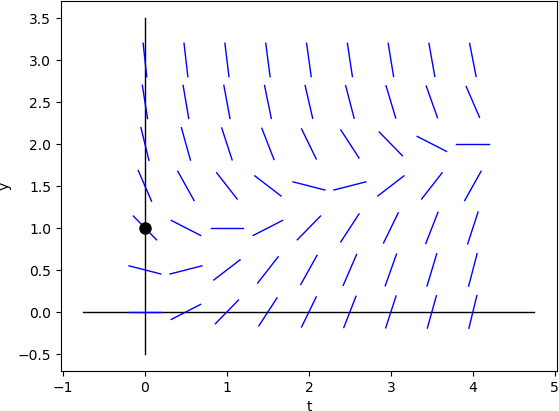
\includegraphics[width=0.31\textwidth]{figs/sequence-1} $\,$
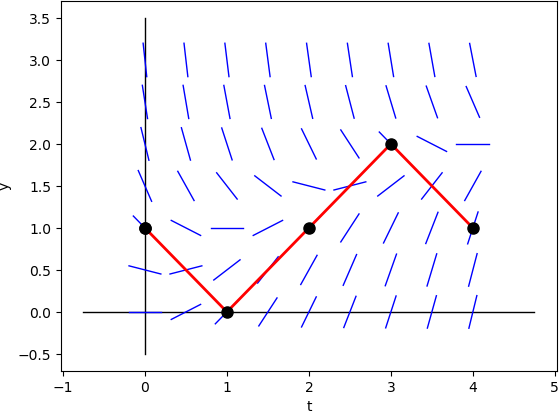
\includegraphics[width=0.31\textwidth]{figs/sequence-2} $\,$
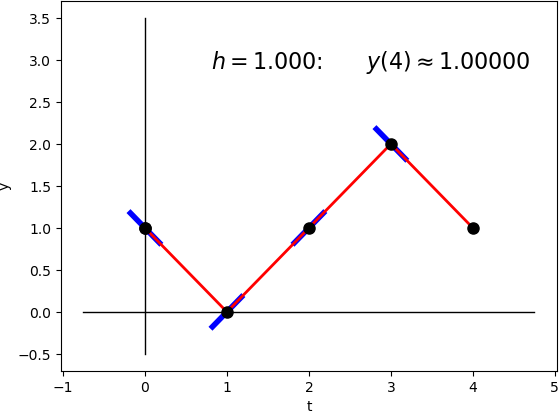
\includegraphics[width=0.31\textwidth]{figs/sequence-3} $\,$
}

\bigskip

\hspace{-12mm} \mbox{
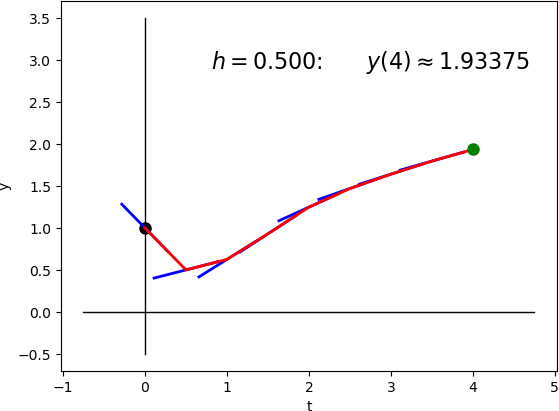
\includegraphics[width=0.31\textwidth]{figs/sequence-4} $\,$
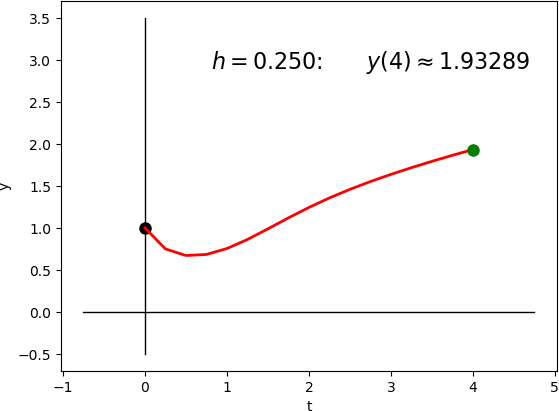
\includegraphics[width=0.31\textwidth]{figs/sequence-5} $\,$
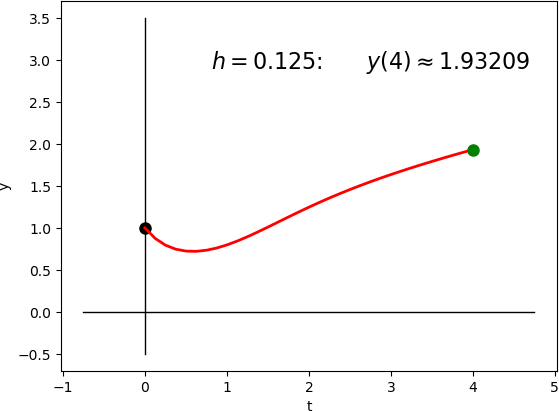
\includegraphics[width=0.31\textwidth]{figs/sequence-6}
}

    \begin{itemize}
    \item this visualization needs to make sense! review Euler's method!
    \end{itemize}
\end{itemize}
\end{frame}


\begin{frame}[fragile]
\frametitle{Euler's method is a short code}

\bigskip
\VerbatimInput[fontsize=\footnotesize]{../codes/euler1.m}
\end{frame}

% for problem:
% >> f = @(t,y) t - y^2;
% >> optt = odeset('RelTol',RTOL,'AbsTol',1.0e-14);
% >> [tt,yy] = ode45(f,[0,4],1,optt); yy(end)
%ans =  1.93122683184240
%       -----------       <- 10 digits which agree for
%                            RTOL=1.0e-9,1.0e-10,1.0e-11,1.0e-12
% will use:  yexact = 1.9312268318427   based on above and RK4 with h=0.0001

\begin{frame}[fragile]
\frametitle{example with \texttt{euler1.m}}

\begin{columns}
\begin{column}{0.55\textwidth}
\begin{itemize}
\item you can run this with \href{https://octave-online.net/}{Octave Online} or \Matlab or \Octave
\item see comments:
\begin{Verbatim}[fontsize=\footnotesize]
>> help euler1
\end{Verbatim}
\item run the example:
\begin{Verbatim}[fontsize=\footnotesize]
>> f = @(t,y) t - y^2;
>> [tt,yy] = euler1(f,[0,4],1,0.5);
>> plot(tt,yy)
\end{Verbatim}
\item reduce step size and overlay:
\begin{Verbatim}[fontsize=\footnotesize]
>> [tt,yy] = euler1(f,[0,4],1,0.25);
>> hold on
>> plot(tt,yy,'r')
\end{Verbatim}
\end{itemize}
\end{column}
\begin{column}{0.45\textwidth}

\mbox{\quad 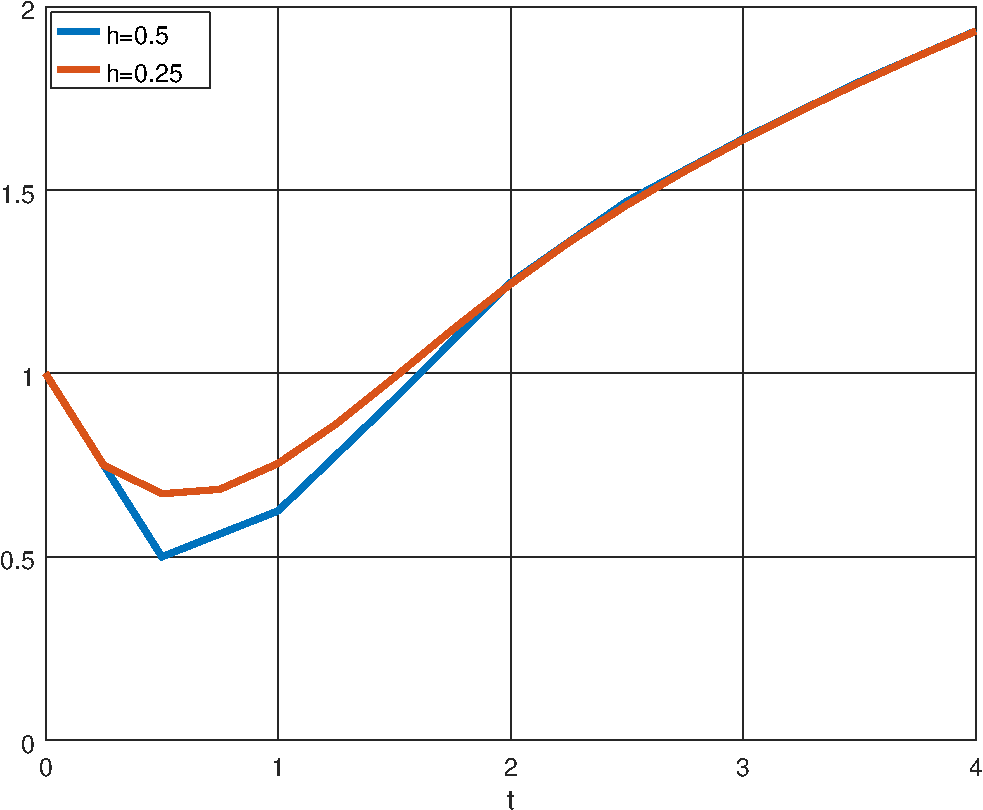
\includegraphics[width=\textwidth]{figs/euler1basic}}
\end{column}
\end{columns}
\end{frame}


\begin{frame}[fragile]
\frametitle{\texttt{euler1.m}: explaining the lines}

\begin{itemize}
\item the top line declares what are inputs and outputs:

{\color{Green}
\begin{Verbatim}[fontsize=\small]
function [t, y] = euler1(f,tspan,y0,h)
\end{Verbatim}
}
    \begin{itemize}
    \item \texttt{tspan} is vector of two numbers: \footnotesize $[t_0,t_f]=$\texttt{[tspan(1),tspan(2)]}
    \end{itemize}
\item then there is a block of comments
\item the first ``real'' line computes the number of steps wanted by user, based on $h$ and $[t_0,t_f]$:  \quad $M=(t_f-t_0)/h$

{\color{Green}
\begin{Verbatim}[fontsize=\small]
M = round((tspan(2)-tspan(1))/h);
\end{Verbatim}
}
\item given the number of steps, values $t_n$ can be pre-computed:

{\color{Green}
\begin{Verbatim}[fontsize=\small]
t = linspace(tspan(1),tspan(2),M+1);
\end{Verbatim}
}
    \begin{itemize}
    \item for example, \texttt{linspace(0,4,5)} is the list $[0,1,2,3,4]$
    \item same as \,\,\texttt{t = tspan(1):h:tspan(2);} \,\, if user is careful
    \end{itemize}

\item allocate empty space for solution: {\color{Green}\texttt{y = zeros(size(t));}}
\item \begin{minipage}[t]{0.3\textwidth}
remainder is Euler's method itself:
\end{minipage}
\quad
\begin{minipage}[t]{0.55\textwidth}
\vspace{-3mm}
{\color{Green}
\begin{Verbatim}[fontsize=\small]
y(1) = y0;
for n = 1:M
    y(n+1) = y(n) + h * f(t(n),y(n));
end
\end{Verbatim}
}
\end{minipage}
\end{itemize}

\end{frame}


\begin{frame}[fragile]
\frametitle{from Euler to \texttt{ode45} in three steps}

\begin{itemize}
\item our use of \texttt{euler1} should look familiar

\begin{Verbatim}[fontsize=\small]
>> f = @(t,y) t - y^2;
>> [tt,yy] = euler1(f,[0,4],1,0.5);
>> plot(tt,yy)
\end{Verbatim}
     \begin{itemize}
     \item just like how we used \texttt{ode45} in \S5.3 and \S4.10
     \end{itemize}
\item I will show three {\color{Green} new codes}:
\color{Green}{
\begin{Verbatim}
function [t,y] = euler1(f,tspan,y0,h)
function [t,y] = improved2(f,tspan,y0,h)
function [t,y] = rk4(f,tspan,y0,h)     % section 9.2
\end{Verbatim}
}

\vspace{-2mm}
\color{Black}{
\begin{Verbatim}
function [t,y] = ode45(f,tspan,y0)
\end{Verbatim}
}
    \begin{itemize}
     \item all have the same inputs and same size outputs:
     \item they approach the black box \texttt{ode45} in quality
     \item only difference versus \texttt{ode45}: it does not require choice of $h$
     \end{itemize}
\end{itemize}
\end{frame}


\begin{frame}{better than Euler}

\begin{itemize}
\item start again with direction field for $y'=f(t,y)=t-y^2$
\item \emph{improved Euler} takes an Euler step of length $h$ to a temporary value $y^\ast$, then averages slopes at the two known points, then uses the average slope for a step of length $h$
\item visual version:
\end{itemize}

\vspace{-3mm}
\hfill 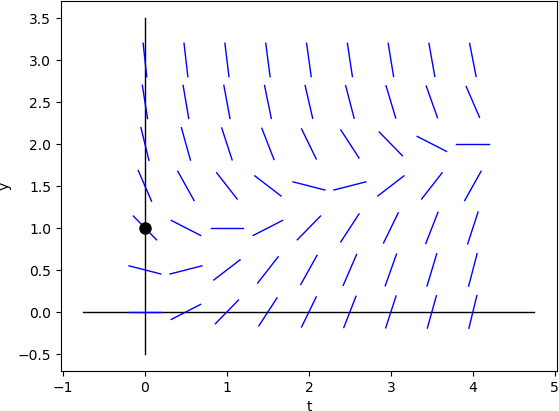
\includegraphics[width=0.7\textwidth]{figs/sequence-1}
\end{frame}


\begin{frame}{\textsl{improved Euler} as formula}

\small
\begin{itemize}
\item it takes an Euler step of length $h$ to a temporary value $y^\ast$
    $$y^\ast = y_n + h f(t_n,y_n)$$
\item \dots then averages slopes at known points
    $$m_{\text{av}} = \frac{1}{2} \left(f(t_n,y_n) + f(t_{n+1},y^\ast)\right)$$
\item \dots then uses the average slope for a step of length $h$
    $$y_{n+1} = y_n + h\, m_{\text{av}}$$
\item thus:
\begin{empheq}[box=\fbox]{align*}
    y^\ast  &= y_n + h f(t_n,y_n) \\
    y_{n+1} &= y_n + \frac{h}{2}\, \left[f(t_n,y_n)+f(t_{n+1},y^\ast)\right]
\end{empheq}
\item or (ugly):
$$y_{n+1} = y_n + \frac{h}{2}\, \left[f(t_n,y_n)+f\left(t_{n+1},y_n+hf(t_n,y_n)\right)\right]$$
\end{itemize}
\end{frame}



\begin{frame}[fragile]
\frametitle{new code just like the old code}

\begin{itemize}
\item my new code \texttt{improved2.m} is just like \texttt{euler1.m}
\item \emph{except} inside the \texttt{for} loop:

\bigskip
{\color{Green}
\begin{Verbatim}[fontsize=\footnotesize]
function [t, y] = improved2(f,tspan,y0,h)
...
for n = 1:M
    ystar = y(n) + h * f(t(n),y(n));
    y(n+1) = y(n) + h * ( f(t(n),y(n)) + f(t(n+1),ystar) ) / 2;
end
\end{Verbatim}
}
\end{itemize}
\end{frame}


\begin{frame}[fragile]
\frametitle{accuracy}

\begin{itemize}
\item let's use a problem where we know the exact solution
\item \emph{example.}  $y' = 1+y^2$, \, $y(0)=0$
\item \emph{exact solution.} it's separable
\footnotesize
\begin{align*}
\int \frac{dy}{1+y^2} &= \int dt \\
\arctan(y) &= t+c \\
y(t) &= \tan t
\end{align*}
\normalsize
\item Euler and improved Euler solutions for $y(1)$ with step $h=0.1$:
\begin{Verbatim}[fontsize=\small]
>> f = @(t,y) 1+y^2;
>> [tt,ye] = euler1(f,[0,1],0,0.1);
>> [tt,yie] = improved2(f,[0,1],0,0.1);
>> ye(end), yie(end), tan(1)
ans =  1.3964
ans =  1.5538
ans =  1.5574
\end{Verbatim}
\end{itemize}
\end{frame}


\begin{frame}[fragile]
\frametitle{plotting style for truth and justice}

\begin{columns}
\begin{column}{0.5\textwidth}
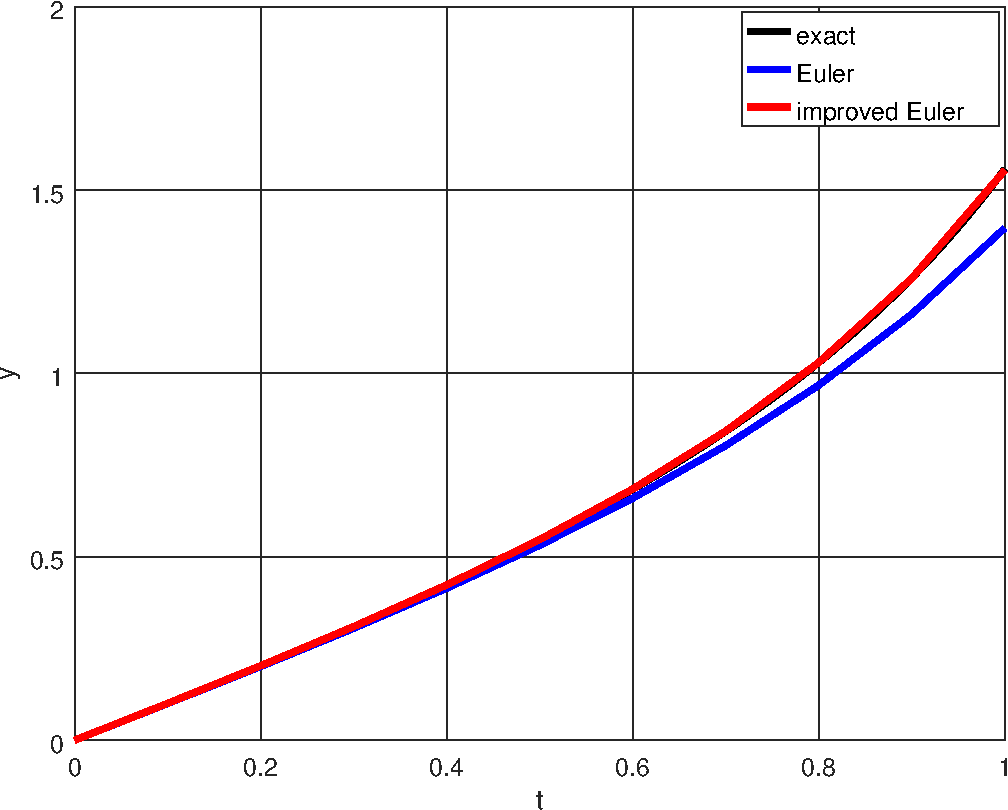
\includegraphics[width=\textwidth]{figs/badstyle}

\begin{Verbatim}[fontsize=\scriptsize]
>> plot(t,yexact,'k',...
        tt,ye,'b',tt,yie,'r')
\end{Verbatim}
\end{column}
\begin{column}{0.5\textwidth}
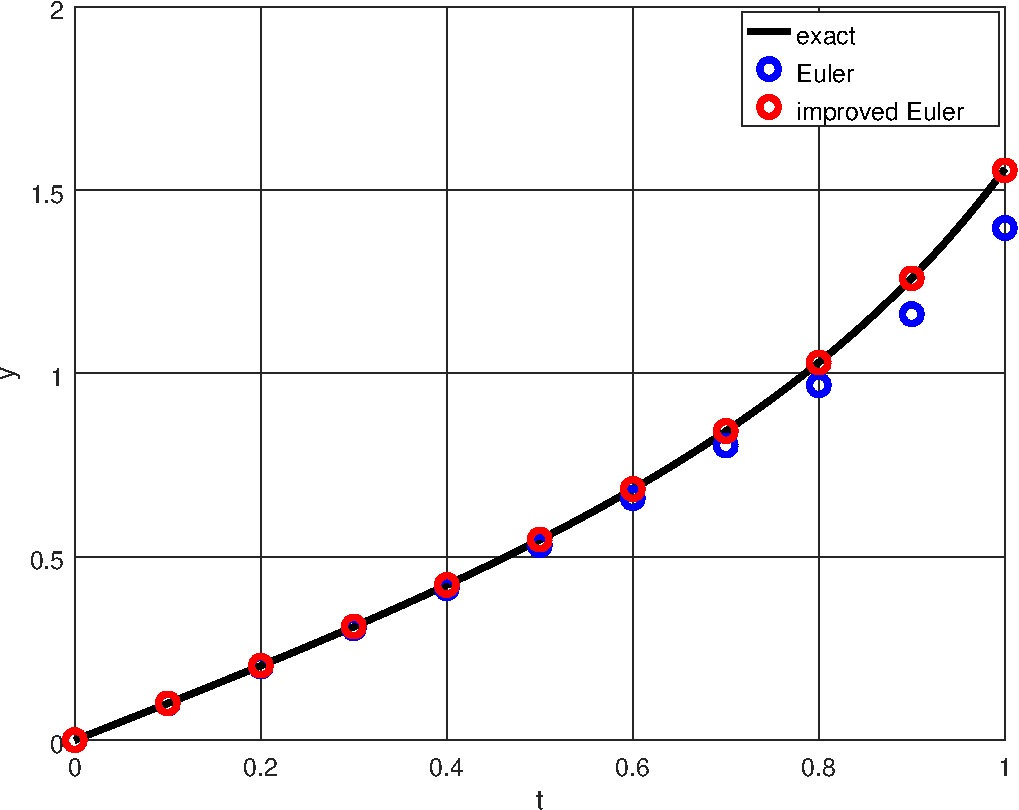
\includegraphics[width=\textwidth]{figs/goodstyle}

\begin{Verbatim}[fontsize=\scriptsize]
>> plot(t,yexact,'k',...
        tt,ye,'bo',tt,yie,'ro')
\end{Verbatim}
\end{column}
\end{columns}
\end{frame}


\begin{frame}{the \S9.1 WebAssign homework is easy}

\begin{itemize}
\item get on \href{https://octave-online.net/}{Octave Online} or \Matlab/\Octave
\item yes, you may and should \emph{use} the codes I have posted at the \href{https://bueler.github.io/math302/codes.html}{Codes tab of the course website}
\item use \texttt{improved2} exactly the way I did two slides back
\item if you have technical difficulties then \emph{post to Piazza}!
    \begin{itemize}
    \item anonymous is fine, but make it a public post for efficiency
    \end{itemize}
\end{itemize}
\end{frame}


\begin{frame}[fragile]
\frametitle{exercise \#9 in \S9.1}

\begin{itemize}
\item \emph{exercise \#9.}  Use the improved Euler's method to obtain a four-decimal approximation of the indicated value.  First use $h=0.1$ and then use $h=0.05$.
    $$y'=xy^2-\frac{y}{x}, \quad y(1)=1; \quad y(1.5)$$

\noindent \emph{solution.} [fill in \Matlab/Octave code]

\vspace{30mm}
%>> f = @(x,y) x*y^2-y/x;
%>> [xx,yy] = improved2(f,[1,1.5],1,0.1);
%>> [xxx,yyy] = improved2(f,[1,1.5],1,0.05);
\begin{Verbatim}[fontsize=\small]
>> yy(end), yyy(end)
ans =  1.3260
ans =  1.3315
\end{Verbatim}
\end{itemize}
\end{frame}

\begin{frame}{regarding exercise \#11}

\begin{itemize}
\item only one part of the WebAssign is not that easy \dots
\item how do you find the ``actual value $y(0.5)$'' for this ODE IVP?
    $$y'=(x+y-1)^2, \, y(0)=2$$
\item \alert{answer.}  we have not solved this kind of ODE before.  but if you substitute $u=x+y-1$ you can work it out
\end{itemize}
\end{frame}


\begin{frame}{notation}

\begin{itemize}
\item one way to derive Euler method is using Taylor series

      \dots but we need clarity about notation first
\item consider $y'=f(t,y)$, as usual, with solution $y(t)$
\item notation:

\vspace{-6mm}
\begin{align*}
y(t) &= \text{(the exact solution)} \\
y(t_n) &= \text{(the exact solution evaluated at $t_n$)} \\
y_n &= \text{(the number computed by numerical method)}
\end{align*}
\item key point about notation:

\medskip
\centerline{\alert{$y(t_n)$ is not the same as $y_n$} \hspace{40mm}}

\medskip
\item absolute error $=|y_n-y(t_n)|$
\end{itemize}

\vspace{-20mm}
\hfill 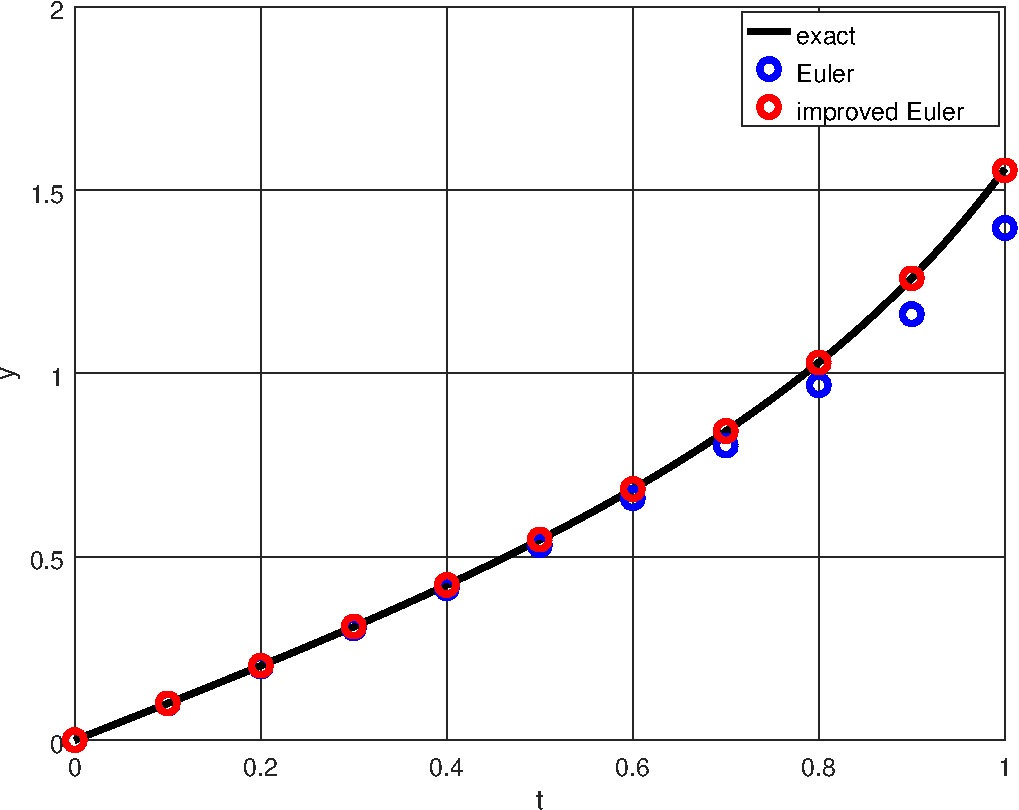
\includegraphics[width=0.4\textwidth]{figs/goodstyle}
\end{frame}


\begin{frame}{order}

\begin{itemize}
\item one may derive Euler method using Taylor series:
   $$y(t+h) = y(t) + y'(t) h + \frac{y''(c)}{2} h^2$$
\item or equivalently, because $t_{n+1} = t_n+h$ and $y'=f(t,y)$:
   $$y(t_{n+1}) = y(t_n) + h\, f(t,y(t_n)) + \frac{y''(c)}{2} h^2$$
\item drop the remainder term; use result to \emph{define} the next value:
   $$y_{n+1} = y_n + h\, f(t,y_n)$$
\item Euler's method is \emph{order 1} because we dropped the ``$h^2$'' term
\item improved Euler method is \emph{order 2} because one may derive it by dropping a ``$h^3$'' term from the Taylor series
    \begin{itemize}
    \item not shown
    \end{itemize}
\end{itemize}
\end{frame}


\begin{frame}{\emph{improved} versus \emph{modified} Euler}

\small
\begin{itemize}
\item in \S2.6 slides I mentioned the \emph{modified} Euler method:

\vspace{-3mm}
\begin{minipage}{0.5\textwidth}
\begin{align*}
    y^\ast  &= y_n + \frac{h}{2} f(t_n,y_n) \\
    y_{n+1} &= y_n + h\, f(t_n+\frac{h}{2},y^\ast)
\end{align*}
\end{minipage}
\hspace{50mm}
\item compare \emph{improved} Euler method (\S9.1):

\vspace{-3mm}
\begin{minipage}{0.5\textwidth}
\begin{align*}
    y^\ast  &= y_n + h f(t_n,y_n) \\
    y_{n+1} &= y_n + \frac{h}{2}\, \left[f(t_n,y_n)+f(t_{n+1},y^\ast)\right]
\end{align*}
\end{minipage}
\hspace{50mm}
\item \alert{\emph{exercise.} sketch each method to the right}
\item alternate (better) naming scheme:

\begin{center}
\begin{tabular}{c|c|c}
\emph{name} & \emph{order} & \emph{alternate name} \\ \hline
Euler & 1 & explicit first-order \\
improved Euler & 2 & explicit trapezoid \\
modified Euler & 2 & explicit midpoint
\end{tabular}
\end{center}
\end{itemize}
\end{frame}


\begin{frame}{comment, and expectations}

\begin{itemize}
\item it turns out that both improved Euler and modified Euler are order 2 methods from the big \emph{Runge-Kutta} family of methods
     \begin{itemize}
     \item \S9.2 introduces an order 4 Runge-Kutta method
     \end{itemize}

\bigskip
\item just watching this video is \emph{not} enough!
     \begin{itemize}
     \item see ``found online'' videos and stuff at

     \centerline{\href{https://bueler.github.io/math302/week10.html}{\tt \color{cyan} bueler.github.io/math302/week10.html}}
     \item \emph{read} section 9.1 in the textbook
     \item \emph{do} the WebAssign exercises for section 9.1
     \end{itemize}
\end{itemize}
\end{frame}

\end{document}

